\documentclass[11pt, oneside]{article}   	% use "amsart" instead of "article" for AMSLaTeX format
\usepackage{geometry}                		% See geometry.pdf to learn the layout options. There are lots.
    \geometry{
     a4paper,
     top=20mm,
     }
\usepackage{hyperref}
\usepackage{amsmath}
\usepackage{underscore}
\usepackage{caption}
\usepackage{algorithmic}
\usepackage{enumitem}	
\usepackage{verbatim}
\usepackage{tikz}				% package for drawing node diagrams for search derivations
\usetikzlibrary{trees}

\def\infinity{\rotatebox{90}{8}}

\hypersetup{
    colorlinks=true,
    linkcolor=blue,
    filecolor=magenta,      
    urlcolor=cyan,
}
\setlength{\parskip}{1em}
\setlength{\parindent}{4em}
\usepackage{graphicx}				% Use pdf, png, jpg, or eps§ with pdflatex; use eps in DVI mode
								% TeX will automatically convert eps --> pdf in pdflatex		
\usepackage{amssymb}

\newenvironment{cmr}{\fontfamily{cmr}\selectfont}{\par}

\setlength{\parskip}{1em}
\setlength{\parindent}{4em}

\title{\vspace{40mm}CPSC 433 --- Assignment I}
\author{
	Daniel Gillson\\
	David Keizer\\
	Ethan Higgs\\
	Zheng Liang\\
	Zibin Mei}
\date{October 20\textsuperscript{th} 2017}

\newpage
\begin{document}
\maketitle
\break

\centerline{{\Large Search Paradigm I --- Set-Based Search}}

\noindent {\\ \large \textbf{Solution Overview}}\\\\
\begin{cmr}
\indent Our approach to solving the problem within the context of set-based search will rely mainly on the use of a genetic algorithm.
We will obtain an initial, randomly generated population for our GA via an Or-tree-based Search that will provide candidate solutions to the problem's
hard constraints. In this first stage of our solution, we ignore the problem's soft constraints, thereby re-formulating it as a constraint satisfaction problem (CSP).

\indent Once we have obtained an initial population of some size, pop_init, we will consider its individuals to be facts in a Set-based Search.
We will also define a constant, pop_max, as an upper bound on the size of any later generation.
The set-based search will use our genetic algorithm's cross-over/mutation function, and a reduce function as its extension rules.
f\textsubscript{Wert} will be used to decide which extension rule to apply.
When the population has exceeded pop_max, f\textsubscript{Wert} will indicate that a reduction is to take place.
f\textsubscript{Select} will be used to determine which two facts to use as parents when applying the cross-over/mutation extension rule.
The start state will be our initial set of randomly generated facts and our end condition will be a predetermined number of generations or a predetermined time limit, whichever comes first.

\indent In our GA, we will use \textbf{Eval} to measure how the well each fact meets soft constraints, \textbf{Constr} and \textbf{Constr\textsuperscript{*}}to check hard constraints, and roulette-wheel selection as a selection method for cross-over/mutation.
\textbf{Constr\textsuperscript{*}} is a variant of \textbf{Constr} used to evaluate the constraint-compliance of partial solutions, which we assume can be derived from the provided \textbf{Constr} function.
\end{cmr}

\noindent {\large \textbf{Or-tree-based Search Model}}

\noindent We define Prob as a vector of length $\vert$Courses + Labs$\vert$, whose elements consist of the indices of slots from Slots, or the unassigned symbol, \$. The vector's ordering will preserve the original ordering of Courses + Labs. Therefore, a Prob vector can be read sequentially as: Course/Lab at position $i$, having value $j$, has been assigned time slot $s_j$, where $s_j$ is the member $s$ of the set Slots at the $j$\textsuperscript{th} index of that set. As such, our definition of Prob is equivalent with the notion of a partial assignment, \textit{partassign}.

\noindent Before formally defining Prob, we define $D_i$, the domain of any element in a problem instance, pr, to be the set: \{0, $\dots$, $j$\} where $j+1$ = $\vert$Slots$\vert$.

\noindent \centerline{Prob =  $\langle C_1 \text{slot}, \dots, C_n \text{slot}, \dots, L_{11} \text{slot}, \dots, L_{1{k_1}} \text{slot}, \dots, L_{n1} \text{slot}, \dots, L_{n{k_n}} \text{slot}\rangle$}\\
\centerline{such that $C_i \text{slot}$, $L_{i{k_i}} \text{slot} \in D_i \cup \{\$\}$}

\noindent Which can be abstracted into the form:

\noindent \centerline{Prob = $\langle X_1, \dots, X_n\rangle$ such that $X_i \in D_i \cup \{\$\}$}

\noindent We define our alternatives relation, Altern, as follows:

\noindent \centerline{Altern = $\{(\langle X_1, \dots, X_i, \dots, X_n \rangle, \langle X_1, \dots, d_{i1}, \dots, X_{in} \rangle, \dots, \langle X_1, \dots, d_{i\ell}, \dots, X_n \rangle)$ $\vert$ $X_i$ = $\$$,}\\
\centerline{$1 \le i \le n$, $\vert D_i \vert = \ell$, $D_i = \{d_i, \dots, d_{i\ell}\}\}$}

\noindent We define the notion, ``pr is solved" as follows:

\noindent \centerline{pr = $\langle X_1, \dots, X_n \rangle$ and $\forall i$ such that $1 \le i \le n$, $X_i$ $\neq$ $\$$, and pr is not unsolvable.}

\noindent We define the notion, ``pr is unsolvable" as follows:

\noindent \centerline{pr = $\langle X_1, \dots, X_n \rangle$ and \textbf{Constr\textsuperscript{*}}(pr) = false.}

\noindent Since we have access to \textbf{Constr\textsuperscript{*}}, derived from the provided function, \textbf{Constr}, we can allow \textbf{Constr\textsuperscript{*}} to perform the work of assessing whether any particular problem instance, pr, is compliant with the problem's hard constraints.

\noindent {\large \textbf{Or-tree-based Search Process}}

\begin{cmr}
\noindent Initial Search Control:

\noindent This is the search control for the generation of the initial population for the set-based search.

\noindent Our O\textsubscript{Tree} will begin with a single node, (pr, ?). Its expansion will be governed by the recursive relation, Erw\textsubscript{$\lor$}.
If a partial assignment is provided, pr, is of the form \textit{partassign} and expansion will begin at the first \$ in pr. For all subsequent assignments, the search control will replicate the form of \textit{partassign} wherever it had made an assignment.

\noindent In general, the search control will construct pr in a left to right fashion, assigning slots to elements of pr from the lowest to the highest index.

\noindent In order to decide which leaf to operate on, the search control applies f\textsubscript{leaf}. It first looks for leaf nodes where the problem is solvable. If there are multiple of these leaf nodes, then one is chosen at random. The sol-entry of the selected node is then changed to ``Yes'' and the search is finished.

\noindent If no such leaf nodes exist, then the search control considers any leaf nodes where the problem is unsolvable. If there are multiple of these nodes, then they are processed from left to right --- updating their sol-entries to ``No''.

\noindent If neither of these types of leaf nodes exist, then the search control selects the leaf which has the fewest unassigned courses/labs (\$'s) --- therefore the deepest leaf node in the tree. 
There will always be multiple of these nodes, since the search control works one element at a time, so one will need to be chosen randomly and Altern will be applied to this node.

\noindent In order to define f\textsubscript{leaf}, we must first define a function, sum\$: pr $\Rightarrow$ $\mathbb{Z}$. Which, given some pr, returns the number of \$ entries within it. 

\noindent Given,\\
\centerline{P =  \{\{pr\textsubscript{1}, $\dots$, pr\textsubscript{$k$}\} $\vert$ sum$\$$(pr\textsubscript{$i$}) = sum$\$$(pr\textsubscript{$j$}), 1 $\leq$ $i$, $j$ $\leq$ $k$, $i \neq j$ \}}

\noindent We define a function rand: pr $\Rightarrow$ $\mathbb{R}$ to deal with multiple deepest leaf nodes.

\noindent Let $z$ be a random integer such that 1 $\leq$ $z$ $\leq$ $\vert$P$\vert$. Then,\\
 
     \[
         \text{rand} = \left\{\begin{array}{ll}
             0 & \text{: pr\textsubscript{$z$}}\\
             0.01 & \text{: pr\textsubscript{$i$} $\vert$ $i$ $\neq$ $z$, 1 $\leq$ $i$ $\leq$ $\vert$P$\vert$}\\
             \end{array}\right\}
       \]


\end{cmr}

\noindent Here  pr\textsubscript{$i$} = \{X\textsubscript{1}, $\dots$, X\textsubscript{$n$}\} and input is a \textit {partassign} = \{y\textsubscript{1}, $\dots$, y\textsubscript{$n$}\}, which is either the \textit{partassign} given to the search as the input or s\textsubscript{0}, as defined the the search instance.

\noindent Now we define f\textsubscript{leaf}: pr\textsubscript{$i$} $\Rightarrow$ $\mathbb{R}$\\
    \[
        \text{f\textsubscript{leaf}} = \left\{\begin{array}{ll}
            -1 & \text{: pr\textsubscript{$i$} is solvable}\\
            0 & \text{: pr\textsubscript{$i$} is unsolvable}\\
            \text{sum$\$$(pr\textsubscript{$i$}) + rand(pr\textsubscript{$i$})} & \text{: $\forall X\textsubscript{i}$ = y\textsubscript{i} or y\textsubscript{i} = \$}
            \end{array}\right\}
      \]

\begin{cmr}
\noindent At each tree depth, our search control will apply the process described above in order to either continue the expansion of O\textsubscript{Tree}, or return a solution.
\end{cmr}

\noindent {\large \textbf{Or-tree-based Search Instance:}}

\noindent We define our initial search state, $s_0$, as follows:

\noindent \centerline{$s_0$ = pr = $\langle X_1, \dots, X_n\rangle$ such that, $\forall X_i$ $\in$ pr, $X_i$ = \$}

\noindent However, $s_0$ will occasionally be equal to a partial assignment, \textit{partassign}.

\noindent Our goal state, $G_{\lor}$, is equivalent with the definition of the notion, ``pr is solved", as seen above.\\
\newpage

\noindent {\large \textbf{Set-based Search Model}}

\begin{cmr}
\noindent We define a set of facts, $F$, to be a set of candidate solutions produced by an Or-tree-based Search as described above.
As mentioned in the problem overview, we will assume that our initial set $F$ will be of size pop_init.
\end{cmr}

\noindent Before formally defining $F$, we define $D_i$, the domain of any element in an individual, $F_i$, to be the set: \{0, $\dots$, $j$\} where $j+1$ = $\vert$Slots$\vert$.

\noindent \centerline{$F$ = \{$\langle X_1, \dots, X_n\rangle$\textsubscript{$1$}, $\dots$, $\langle X_1, \dots, X_n\rangle$\textsubscript{$k$} $\vert$ $X_i \in D_i$, $1 \le i \le n$, $k = \text{pop_init}$\}}

\noindent Before defining Ext, we will first define an alternative Search Control for the Or-tree-based Search which will be applied when using the cross-over/mutation extension rule.

\noindent Search Control\textsubscript{Alt}:

\noindent Our O\textsubscript{Tree}, once again, will begin with a single node, (pr, ?); and its expansion will be governed by the recursive relation, Erw\textsubscript{$\lor$}.

\noindent If both of the selected parents, $A$ and $B$, have the same first element, then pr will be initialized with that element's value as its first element, followed by \$'s. Otherwise pr will be initialized with all \$'s, as before.

\noindent The only difference between Search Control\textsubscript{Alt} and the initial search control is that the two parents must be considered in f\textsubscript{leaf}.

\noindent As such, we redefine the set P used by the rand function as follows:\\\\
\centerline{P =  \{\{pr\textsubscript{1}, $\dots$, pr\textsubscript{$k$}\} $\vert$ sum$\$$(pr\textsubscript{$i$}) = sum$\$$(pr\textsubscript{$j$}),}\\
\centerline{(X\textsubscript{$i$\textsubscript{$\ell$}} = par\textsubscript{1\textsubscript{$\ell$}} or X\textsubscript{$i$\textsubscript{$\ell$}} = par\textsubscript{2\textsubscript{$\ell$}} and X\textsubscript{$j$\textsubscript{$\ell$}} = par\textsubscript{1\textsubscript{$\ell$}} or X\textsubscript{$j$\textsubscript{$\ell$}} = par\textsubscript{2\textsubscript{$\ell$}}, or }
\centerline{X\textsubscript{$i$\textsubscript{$\ell$}} $\neq$ par\textsubscript{1\textsubscript{$\ell$}} and X\textsubscript{$i$\textsubscript{$\ell$}} $\neq$ par\textsubscript{2\textsubscript{$\ell$}} and X\textsubscript{$j$\textsubscript{$\ell$}} $\neq$ par\textsubscript{1\textsubscript{$\ell$}} and X\textsubscript{$j$\textsubscript{$\ell$}} $\neq$ par\textsubscript{2\textsubscript{$\ell$}}), and}\\
\centerline{1 $\leq$ $i$, $j$ $\leq$ $k$, $i \neq j$ \}}

\noindent Where $\ell$ is the index of the pr's under consideration at the current tree depth. By our definition, P will either contain all the leaf nodes where the value of the $\ell$'th element matches one of the two parents, or P will contain all the leaf nodes where no match is found.

\noindent We denote the parents as follows:\\\\
\centerline{Par\textsubscript{1} = \{par\textsubscript{1\textsubscript{1}}, $\dots$, par\textsubscript{1\textsubscript{$n$}}\} and Par\textsubscript{2} = \{par\textsubscript{2\textsubscript{1}}, $\dots$, par\textsubscript{2\textsubscript{$n$}}\}}

\noindent If both parent elements at the position under consideration constitute valid additions to pr, one will be chosen randomly, according to f\textsubscript{leaf}. Otherwise, if neither parent element would be a valid addition to pr, a valid option generated by Altern will be chosen randomly.
     \[
         \text{f\textsubscript{leaf}} = \left\{\begin{array}{ll}
             -1 & \text{: (pr\textsubscript{$i$} is solved)}\\
             0 & \text{: (pr\textsubscript{$i$} is unsolvable)}\\
             \text{sum$\$$(pr\textsubscript{$i$})+ rand(pr\textsubscript{$i$})} & \text{: X\textsubscript{$i$} = par\textsubscript{1\textsubscript{$i$}} or X\textsubscript{$i$} = par\textsubscript{2\textsubscript{$i$}}}\\
             \text{sum$\$$(pr\textsubscript{$i$})+ rand(pr\textsubscript{$i$})} + 0.1 & \text{: X\textsubscript{$i$} $\neq$ par\textsubscript{1\textsubscript{$i$}} and X\textsubscript{$i$} $\neq$ par\textsubscript{2\textsubscript{$i$}}}\\
 	\infty & \text{: else}
             \end{array}\right\}
       \]

\noindent Now we will define the set of extension rules, Ext:
\begin{enumerate} [topsep=0pt, itemsep=0pt, leftmargin=*]
\item Cross-Over/Mutation:
	\begin{enumerate}[leftmargin=*]
	\item $A$ = f\textsubscript{select}($F$), $B$ = f\textsubscript{select}($F - A$). (We will define f\textsubscript{select}($F$) in our Search Process).
	\item Now that we have selected two parent facts, we will execute our Or-tree-based Search using Search Control\textsubscript{Alt}.
	\item The resulting solution produced by this search will then be added to the population.
	\end{enumerate} 
\item Reduce:
	\begin{enumerate}
	\item The set $F$ is sorting according to \textbf{Eval}: sort($F$, \textbf{Eval})
	\item The first individual in $F$ is then removed: $F$ = $F$ - $F_0$
	\item This brings the size of $F$ back down to pop_max, since we only ever add a single individual at a time.
	\end{enumerate}
\end{enumerate}

\noindent {\large \textbf{Set-based Search Process}}

\noindent Here we define the function, f\textsubscript{select}($F$), which will be used in Ext to pick individuals out of the population in order to perform the crossover operation on them.

\noindent f\textsubscript{select}: $F$ $\Rightarrow$ ($F_i$) is an implementation of the roulette-wheel selection algorithm.\\\\
f\textsubscript{select}($F$) \{
\begin{algorithmic}[\textfloatsep = 0pt]
    \STATE sum = 0
    \FOR {$A_i$ in $F$}
    	\STATE $A_i$.\textbf{Eval} = \textbf{Eval}($A_i$)
	\STATE sum ++ $A_i$.\textbf{Eval}
    \ENDFOR
    \FOR {$A_i$ in $F$}
    	\STATE $A_i$.\textbf{Eval}_norm = $A_i$.\textbf{Eval} / sum
    \ENDFOR
    \STATE sort($F$, $A_i$.\textbf{Eval}_norm)
    \FOR {$A_i$ in $F$}
    	\FOR {$A_j$ in $F$ and $A_j$.index $<$ $A_i$.index}
    		\STATE $A_i$.ACNF += $A_j$.\textbf{Eval}_norm
    	\ENDFOR
    \ENDFOR
    \STATE rand r = randFloatBetween(0, 1)
    \STATE selected = NULL
    \STATE index = 0
    \WHILE {true}
    	\STATE selected = $F_{\text{index}}$
    	\IF {$F_{\text{(index + 1)}}$.ACNF $\geq$ r}
    		\STATE return selected
    	\ENDIF
	\STATE index ++ 1
    \ENDWHILE \\ \}
\end{algorithmic}
      
\noindent Search Control:

\noindent The search control for our Set-based Search will be responsible for producing the initial set, $F$, tracking the amount of time elapsed, and counting the number of generations that our GA has modelled. The first thing our control will do is start a timer.

\noindent In order to produce $F$, the control will execute the following algorithm:

\noindent produce($F$) \{
\begin{algorithmic}[\textfloatsep = 0pt]
    \STATE $i$ = 0
    \WHILE {$i <$ pop_init}
    	\IF {\textit{partassign} $\in$ input}
		\STATE individual = Or-tree-based Search execution with $s_0$ = \textit{partassign}
	\ELSE
		\STATE individual = Or-tree-based Search execution with $s_0$ as originally defined in our Or-tree-based Search Instance
	\ENDIF
	\STATE $F$ = $F$ + individual
	\STATE $i$ ++ 1
    \ENDWHILE \\ \}
\end{algorithmic}

\noindent Once $F$ has been produced, our GA will begin its work.

\noindent We also define a function pop($F$) which evaluates the size of the current population, where $F$ is the current set of facts.
 
     \[
         \text{pop(F)} = \left\{\begin{array}{ll}
             -1 & \text{: $\vert$F$\vert$ $>$ pop_max}\\
             1 & \text{: else}
             \end{array}\right\}
       \]

\noindent In order to decide which transition to apply to our set of facts we pick the transition that minimizes f\textsubscript{Wert}.
 
     \[
         \text{f\textsubscript{Wert}(A, B, e)} = \left\{\begin{array}{ll}
             \text{pop(F)} & \text{: B = $F - F_0$}\\
             0 & \text{: B = else }
             \end{array}\right\}
       \]

\noindent f\textsubscript{Wert} evaluates to -1 if the transition under consideration is reduce and the size of the current generation is larger than pop_max.
It evaluates to 1 when considering reduce and the current generation is not too large.
Lastly, f\textsubscript{Wert} evaulates to 0 whenever the cross-over/mutate rule is being considered.

\noindent Each time the cross-over/mutate rule is applied, the generation counter will increase by 1. If after any application of an extension rule, the time limit is up or the generation counter reaches the predetermined maximum threshold, the search control will halt the GA. At that point, the most fit individual (according to the \textbf{Eval} function) in the current population will be returned as the final, optimized solution to the assignment problem.

\noindent {\large \textbf{Set-based Search Instance}}

\noindent s\textsubscript{0} = Start state for the search instance --- composed of pop_init candidate solutions.\\
G\textsubscript{Set}(s) = Yes, if and only if enough generations have been reached or enough time has elapsed.\\

\noindent That concludes our description of a Set-based Search solution to the assignment problem.
\newpage

\noindent {\large \textbf{A simple example:}}

\noindent Slots = \{$s_1, s_2, s_3$\}, Courses = \{$c_1, c_2$\}, Labs = \{$l_{11}, l_{21}$\}

\noindent Hard Constraints:
\begin{enumerate}[topsep=0pt, itemsep=0pt]
\item \textbf{Constr} and \textbf{Constr\textsuperscript{*}} both equal false if $c_1$ is assigned $s_1$
\item \textbf{Constr} and \textbf{Constr\textsuperscript{*}} both equal false if $l_{21}$ is assigned $s_3$
\end{enumerate}

\noindent Soft Constraints:
\begin{enumerate}[topsep=0pt, itemsep=0pt]
\item \textbf{Eval} and \textbf{Eval\textsuperscript{*}} both equal 5 if $c_1$ is assigned $s_2$
\item \textbf{Eval} and \textbf{Eval\textsuperscript{*}} both equal 5 if $l_{21}$ is assigned $s_1$
\end{enumerate}

\noindent \textbf{Or-tree candidate \#1 search derivation with the initial search control:}

\noindent The values underneath each node are f\textsubscript{leaf} values.

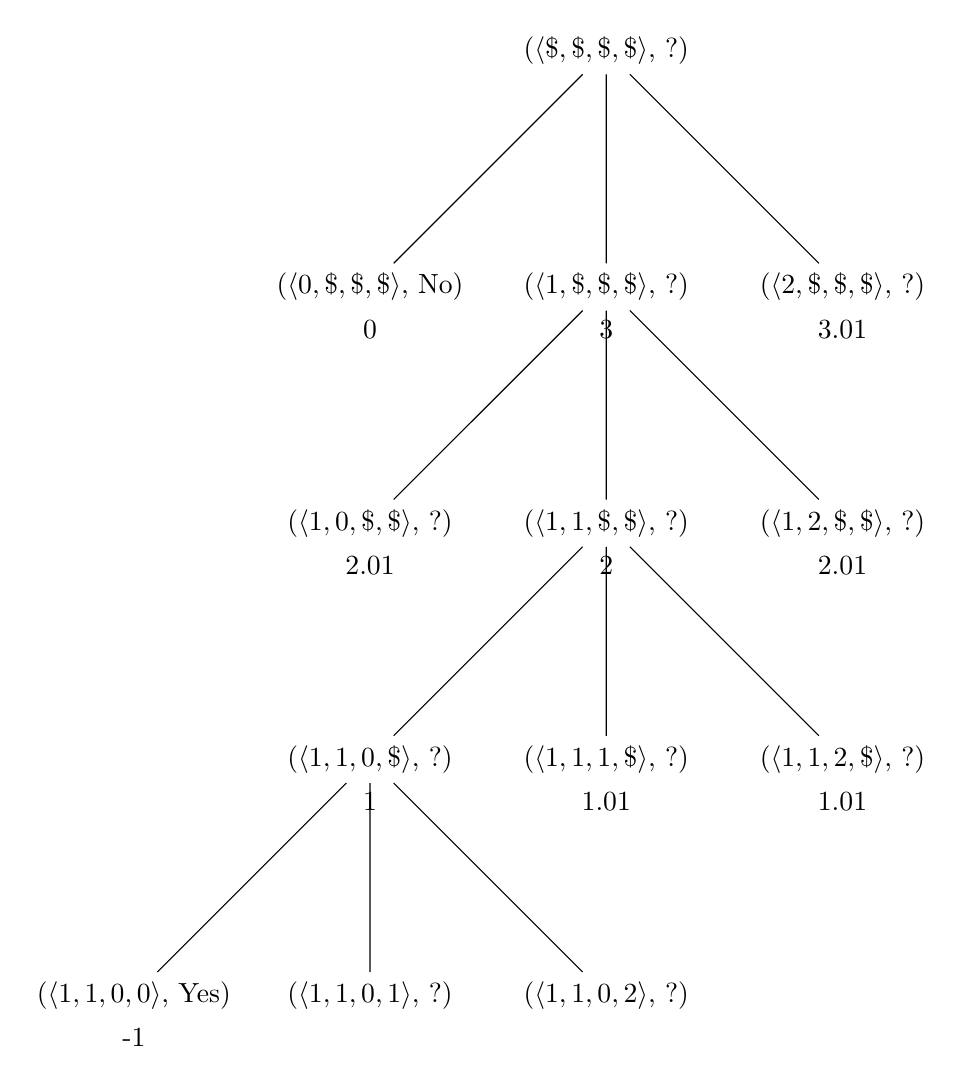
\begin{tikzpicture}[level distance=3cm,
  level 1/.style={sibling distance=3cm},
  level 2/.style={sibling distance=3cm}]
  \node {($\langle \$, \$, \$, \$  \rangle$, ?)}
    child {node[label=below: 0] {($\langle 0, \$, \$, \$  \rangle$, No)} }
    child {node[label=below: 3] {($\langle 1, \$, \$, \$  \rangle$, ?)}
    	child {node[label=below: 2.01] {($\langle 1, 0, \$, \$  \rangle$, ?)}}
      	child {node[label=below: 2] {($\langle 1, 1, \$, \$  \rangle$, ?)}
		child {node[label=below: 1] {($\langle 1, 1, 0, \$  \rangle$, ?)}
			child {node[label=below: -1] {($\langle 1, 1, 0, 0  \rangle$, Yes)}}
		      	child {node {($\langle 1, 1, 0, 1  \rangle$, ?)}}
			child {node {($\langle 1, 1, 0, 2  \rangle$, ?)}} }
	      	child {node[label=below: 1.01] {($\langle 1, 1, 1, \$  \rangle$, ?)}}
		child {node[label=below: 1.01] {($\langle 1, 1, 2, \$  \rangle$, ?)}} }
	child {node[label=below: 2.01] {($\langle 1, 2, \$, \$  \rangle$, ?)}}
    }
    child {node[label=below: 3.01] {($\langle 2, \$, \$, \$  \rangle$, ?)}};
\end{tikzpicture}

\noindent For the sake of brevity, we now assume that we have derived another candidate solution: $\langle 2, 2, 0, 1  \rangle$.
\newpage

\noindent \textbf{Or-tree cross-over/mutation search derivation with Search Control\textsubscript{Alt}:}\\\\
Par\textsubscript{1} = $\langle 1, 1, 0, 0  \rangle$, Par\textsubscript{2} = $\langle 2, 2, 0, 1  \rangle$\\\\
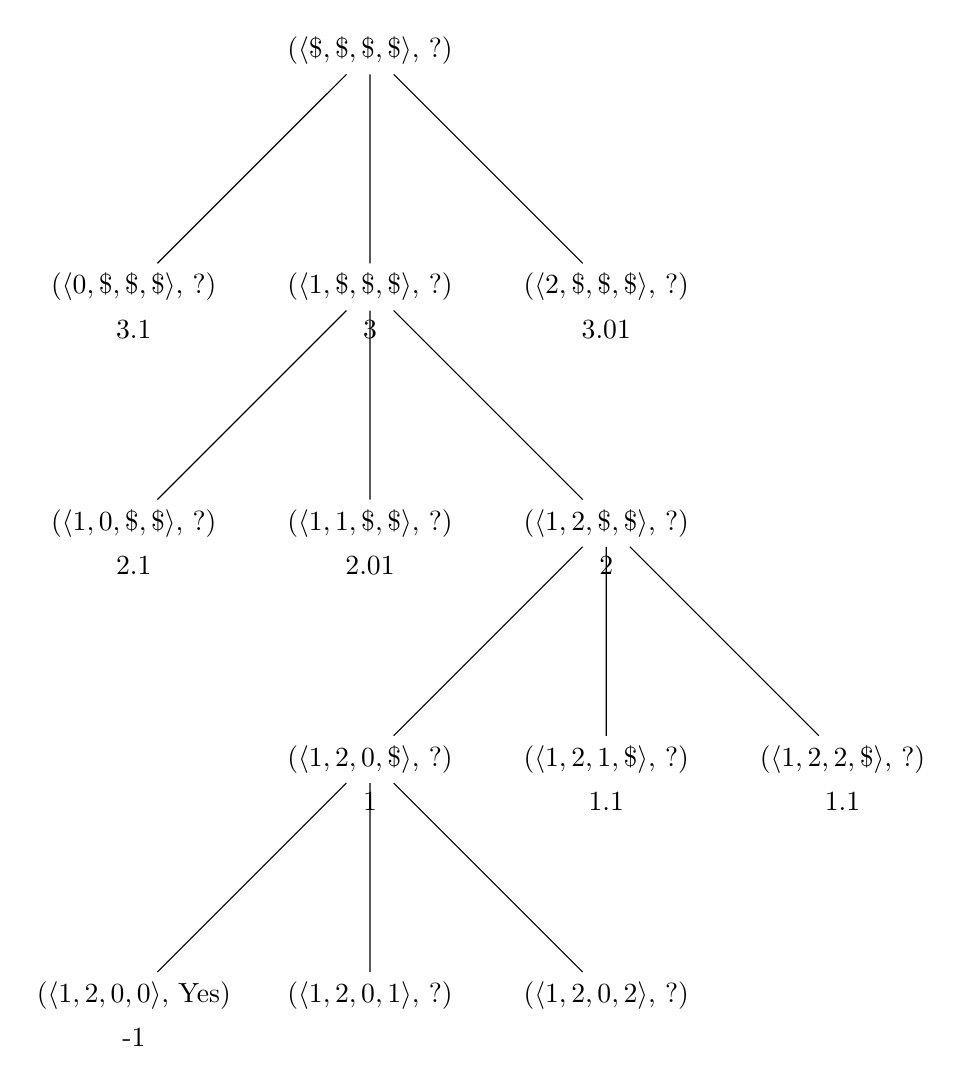
\begin{tikzpicture}[level distance=3cm,
  level 1/.style={sibling distance=3cm},
  level 2/.style={sibling distance=3cm}]
  \node {($\langle \$, \$, \$, \$  \rangle$, ?)}
    child {node[label=below: 3.1] {($\langle 0, \$, \$, \$  \rangle$, ?)} }
    child {node[label=below: 3] {($\langle 1, \$, \$, \$  \rangle$, ?)}
    	child {node[label=below: 2.1] {($\langle 1, 0, \$, \$  \rangle$, ?)}}
      	child {node[label=below: 2.01] {($\langle 1, 1, \$, \$  \rangle$, ?)}}
	child {node[label=below: 2] {($\langle 1, 2, \$, \$  \rangle$, ?)}
		child {node[label=below: 1] {($\langle 1, 2, 0, \$  \rangle$, ?)}
			child {node[label=below: -1] {($\langle 1, 2, 0, 0  \rangle$, Yes)}}
			child {node {($\langle 1, 2, 0, 1  \rangle$, ?)}}
			child {node {($\langle 1, 2, 0, 2  \rangle$, ?)}} }
		child {node[label=below: 1.1] {($\langle 1, 2, 1, \$  \rangle$, ?)}}
		child {node[label=below: 1.1] {($\langle 1, 2, 2, \$  \rangle$, ?)}} }
    }
    child {node[label=below: 3.01] {($\langle 2, \$, \$, \$  \rangle$, ?)}};
\end{tikzpicture}

\noindent According to the Soft Constraints:
\begin{enumerate}
\item \textbf{Eval}($\langle 1, 1, 0, 0  \rangle$) = 10
\item \textbf{Eval}($\langle 2, 2, 0, 1  \rangle$) = 0
\item \textbf{Eval}($\langle 1, 2, 0, 0  \rangle$) = 5
\end{enumerate}

\noindent Therefore, $\langle 2, 2, 0, 1  \rangle$ would be the optimal solution after modelling the GA for a single generation.

\newpage

\centerline{{\Large Search Paradigm II --- And-Tree-Based Search}}

\noindent{\\ \large\textbf{And-tree-based Search Model}}

\noindent For the model, Prob is defined as a vector of length $\vert$Courses + Labs$\vert$, whose elements consist of the indices of slots from Slots, or the unassigned symbol, \$. The ordering of vector will be the same as the original ordering of Courses + Labs. Therefore, a Prob vector can be read sequentially as: Course/Lab at position $i$, having value $j$, has been assigned time slot $s_{j}$, where $s_{j}$ is the member $s$ of the set Slots at the $j^{th}$ index of Slots. As such, the definition of Prob is equivalent with the notion of a partial assignment, $\textit{partassign}$.

\noindent The domain of any element in a problem instance, pr, referred to as $D_{i}$, is defined as the set: \{0, $\dots$, $j$\} where $j$ + 1 = $\vert$Slots$\vert$. With that, Prob is defined as follows:

\begin{center}
{Prob = $\langle$$C_{1}$slot, $\dots$,$C_{n}$slot, $\dots$, $L_{11}$slot, $\dots$, $L_{1k_{1}}$slot, $\dots$, $L_{n1}$slot,  $\dots$, $L_{nk_{n}}$slot$\rangle$ \\ such that $C_{i}$slot, $L_{ik_{i}}$slot $\in D_{i} \cup \big\{\$\big\}$}
\end{center}

\noindent Which can be abstracted into the form:

\begin{center}
{Prob = $\langle$$X_{1}$, $\dots$, $X_{n}$$\rangle$ such that $X_{i} \in D_{i} \cup \big\{\$\big\}$ }
\end{center}
We define our division relation, Div, as follows:\\

\noindent \centerline{Div = $\{(\langle X_1, \dots, X_i, \dots, X_n \rangle, \langle X_1, \dots, d_{i1}, \dots, X_{in} \rangle, \dots, \langle X_1, \dots, d_{i\ell}, \dots, X_n \rangle)$ $\vert$ $X_i$ = $\$$,}\\
\centerline{$1 \le i \le n$, $\vert D_i \vert = \ell$, $D_i = \{d_i, \dots, d_{i\ell}\}\}$}

\noindent We define ``pr is solved" as follows:

\begin{center}
{pr = $\langle$$X_{1}, $\dots$, X_{n}$$\rangle$ and $\forall$$i$ such that $1 \le i \le n$, $X_{i} \neq \$$, and pr is not unsolvable.}
\end{center}

\noindent We define ``pr is unsolvable" as follows:

\begin{center}
{pr = $\langle$$X_{1}, $\dots$, X_{n}$$\rangle$ and \textbf{Constr$^{\ast}$}(pr) = false.}
\end{center}

\noindent Since we have access to \textbf{Constr$^{\ast}$}, derived from the provided function, \textbf{Constr}, we can allow  \textbf{Constr$^{\ast}$} to perform the work of assessing whether any particular problem instance, pr, is compliant with the problem's hard constraints.

%INSERT DAVIDS STUFF%

\end{document}